\chapter{Notes}
\section{Background Reading}
I read the thesis paper \textit{The Remarkable Outflows from the Galactic Microquasar SS433} written by Robert Jeffrey to know the very basic background of SS 433 and the goal of my project. I read \textit{Chandra Guide}, which tells about how all parts of Chandra work, including the high resolution mirror assembly, and Chandra High Energy Transmission Grating. I have been reading three papers published by Herman Marshall that are on the similar topic as my project. The Figure 13. in the 2013 paper is a good reference to look at.  










\section{Chandra Software Process}
At first I used Ciao, an X-ray data analysis software, to get used to the files that I will deal with when proceed the X-ray data. Then I moved to ISIS (Integrated Spectrographic Innovative Software), also an X-ray data analysis software, which supports analysis of high resolution X-ray spectra by combining in one
package tools to query a database of atomic data and plasma emission models. 
From tgcat, I searched "ss 433" in "Quick Search" and downloaded the 1999 obsid 106 Chandra data. The package includes matrix files (RMF and ARF) and pha file. The first thing to do is to create a binned spectrum graph and see if it matches the one that made by the author of the paper. I looked up online manual for ISIS \url{http://space.mit.edu/asc/isis/manual.pdf} and codes written by other people that can operate on the matrix files. \url{http://cxc.harvard.edu/proposer/threads/binary/index.html#simulate.}
I only plotted the spectrums of HEG +1 and HEG -1 (two high-energy gratings beside zeroth order) and the one that combined both of them. \\
The next step would be find the range of interest for MEG, where there are evident emission lines by looking at other papers. After finding the range, I will do the same spectrum plotting process to MEG and we should be able to combine HEG and MEG eventually.

Update: MEG range: 0.4 - 5.0 KeV (31-2.5 A)

10/3\\
I will download the short observation from 
\url{http://cda.harvard.edu/chaser/obsRetrieveEntry.do?obsid=20132} and create RMF and ARF and pha files. 




10/8\\
Tgcat is installed. Under tgcat, bin has three items, chandra-get, download\_obsid, and setup\_obsdir. The directory configuration is done with the shell-script, \textbf{setup\_obsdir}, which may be run independently on already-retrieved Chandra archival data.
Above the directory of the datafile (20132), run setup\_obsdir, and then initiate Ciao to add tools in the path. Run ISIS and .load extract.sh to extract pha, rmf, arf files in 20132.\\\\
Downloaded three files that Hermann made that are used for fitting models. Need to understand what they mean, and find out what codes cannot work out, i.e. add\_order.


10/9\\
Filled the spreadsheet which contains the information of the observation, including the MJD dates, orbital phases, precession phases, and the redshift of the red and the blue shifts.
To find the orbital phases and precession phases, use the c file ss-z.c, plug in the MJD dates and ask for the output of  phi\_o, phi\_p, phi\_n, zred, and zblu. 
We can use zred and zblue to find the observed wavelength of the elements from both jets. The formula is $z = \dfrac{\lambda_{obs} - \lambda_{rest}}{\lambda_{rest}}$.

10/10\\
I made a spectrum using the combination of Heg+1 and Heg-1 and label the elements on the graphs. 

10/11\\
Met Herman and he gave us the add\_order file which makes the code work fine. However, the command r\_plot\_counts(meg) does not work properly. 
In aped\_4Tpar\_alldata\_v4.txt, xaped(1).norm1 means the multiple coefficient of the first plasma of one of the jet (which one?). Parameter 15 ties to 2 means parameter 15 shares the same value with parameter 2. Frozen value are not changing when doing modeling. 

10/12\\
I edited aped\_4Tpar\_alldata\_v4.txt and make the parameters of the second jet not tied to the ones of the first jet (tied-to = 0). The following two graphs show the models when parameters are tied and not tied, respectively.

\begin{figure}[h!]
    \centering
    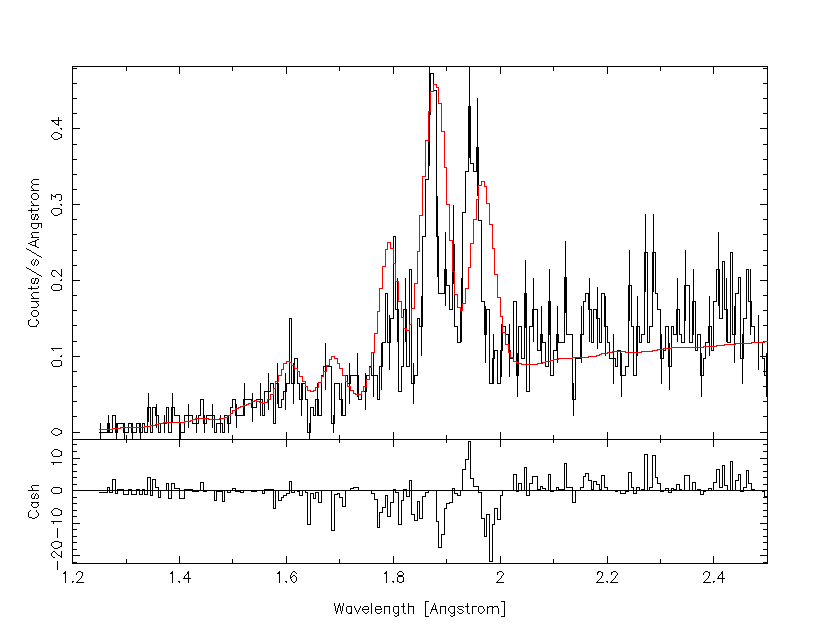
\includegraphics[width=.8\linewidth]{Chapters/Figures/aped_model_tied.png}
    \caption{The aped model with the parameters of two jets tied to each other}
    \label{fig:my_label}
\end{figure}
\newpage
\begin{figure}[h!]
    \centering
    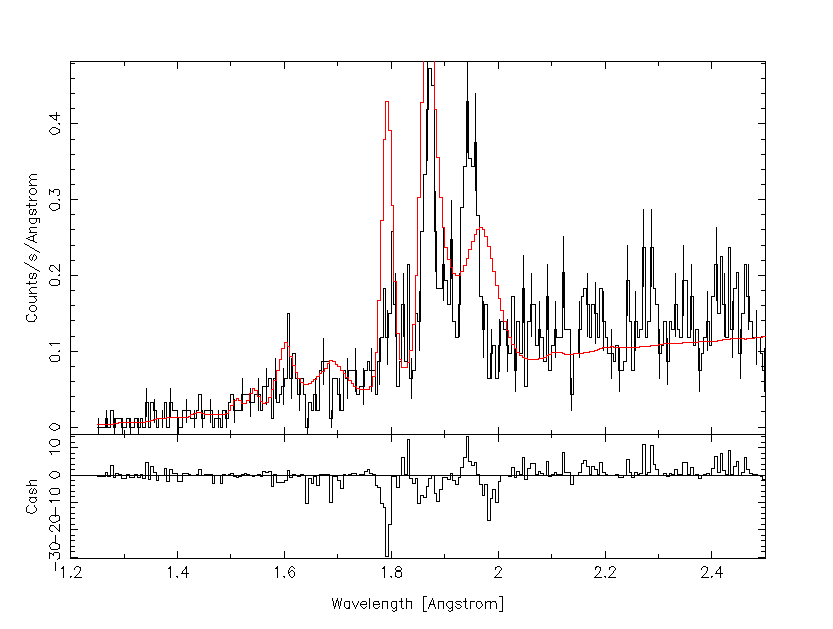
\includegraphics[width=.8\linewidth]{Chapters/Figures/aped_model_untied.png}
    \caption{The aped model with the parameters of two jets not tied to each other}
    \label{fig:my_label}
\end{figure}

10/17\\
Run the fit\_line\_gl4 script, which will produce the gaussian fits for those emission lines. The output files are named as par\_\#lines\_g4.txt. 
The first graph shows almost the same as the one created by fit plasma model script. The only difference is bin number of group\_data is 4 in the current script and is 2 in the plasma script.
Some questions about the fit\_line\_gl4 script.\\
1. Where do the values of line\-wave come from?  Why some line\_wave need to find the average?\\
Update: The line is a blend of two lines and the calculation applies the weights. For example, all lines for H-like ions would be a blend of the alpha1 and alpha2 lines\\
2. conf\_loop generates single-parameter confidence limits for specified parameters (redshift, sigma, rest\_wave.lambda, gaussian properties, etc.) Why it is generating so many files?\\
Update: for each file, it is estimating the parameters by a small regions under the gaussian curve.\\ 
3. What is the difference between the files in conf\_loop and par\_\#lines\_g4.txt?

10/18\\
More questions about fit\_line\_gl4 script.\\
1. What file should go inside load\_par("pars\_all\_lines.txt"); (line 369)? Should it be par\_9lines\_g4.txt?\\
2. How to plot a gaussian plot of just one line?\\
3. Where do those redshift values of two jets come from? Why they are different from the theoretical values? 


10/23\\
Created a new script to plot the fitted line for the spectrum. I moved the plotting command up before the confidence loop and finally got the fitted lines. However, when I changed the redshift to the one that we expect (0.0089 and 0.068), the fitted lines do not catch some important lines. 

10/30\\
To see the line at a certain wavelength is produced by which element and which jet, I plot the graph line by line

First, I plotted the continuum model without fitting any line. See Fig~\ref{fig:continuum}

\begin{figure}[h!]
    \centering
    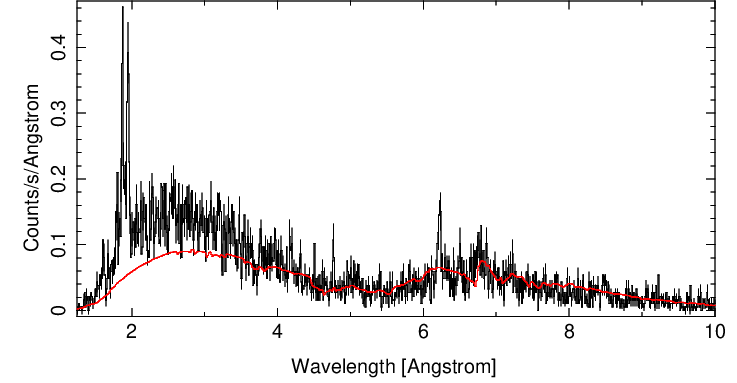
\includegraphics[width=1\linewidth]{Chapters/Figures/unfitted.png}
    \caption{The continuum model prior to fitting lines.}
    \label{fig:continuum}
\end{figure}

The final fitted graph with all lines shows in Fig~\ref{fig:all_lines_1} and Fig~\ref{fig:all_lines_2}

\begin{figure}[h!]
    \centering
    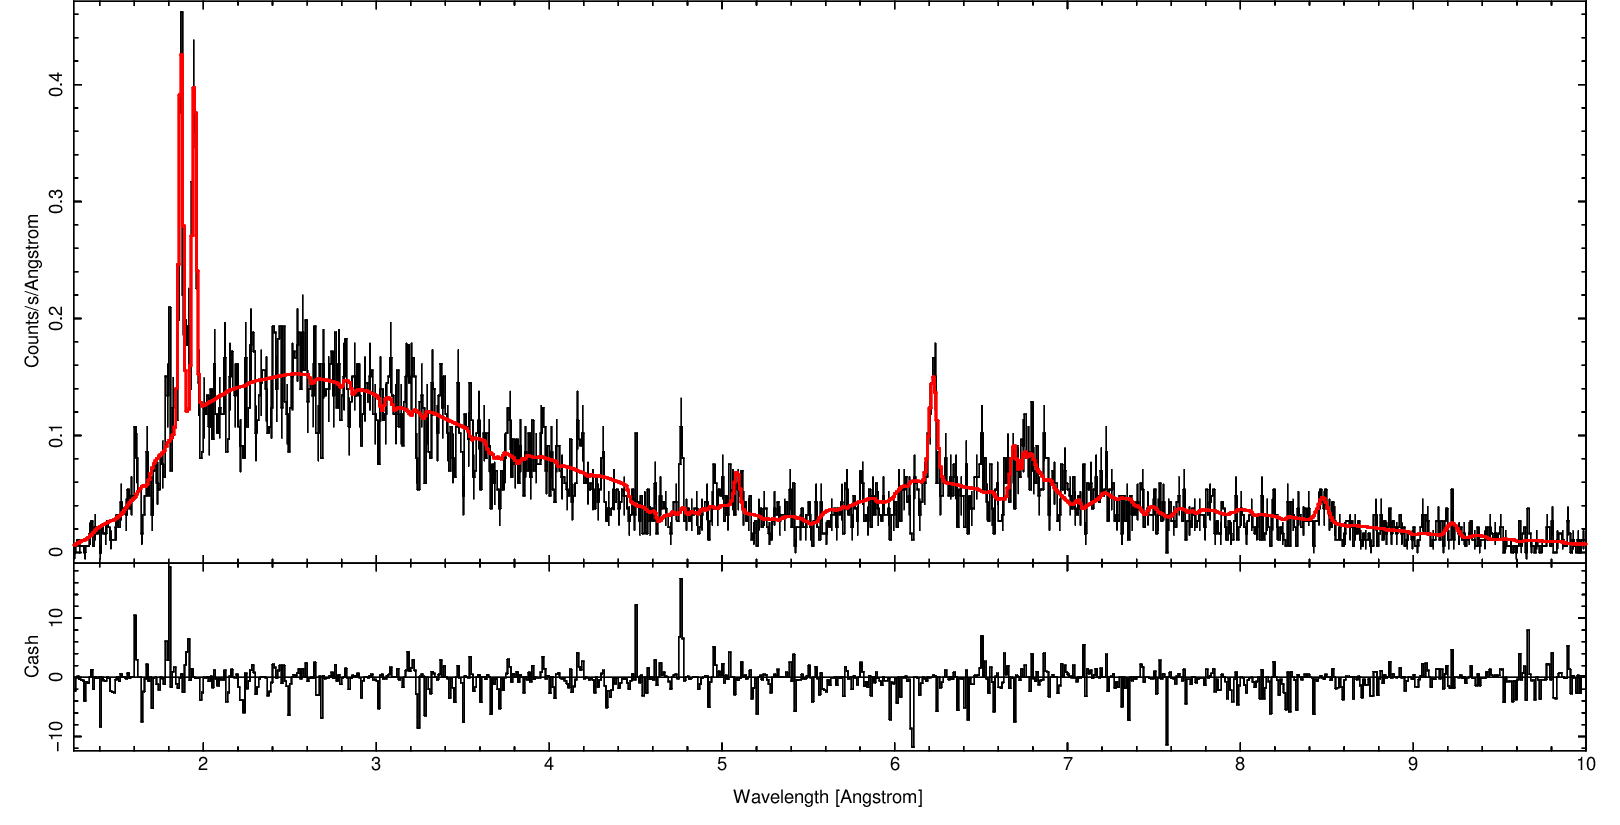
\includegraphics[width=1\linewidth]{Chapters/Figures/all_lines_fitted_heg.png}
    \caption{The fitted lines for the most prominent emissions in the HEG range}
    \label{fig:all_lines_1}
\end{figure}

\begin{figure}[h!]
    \centering
    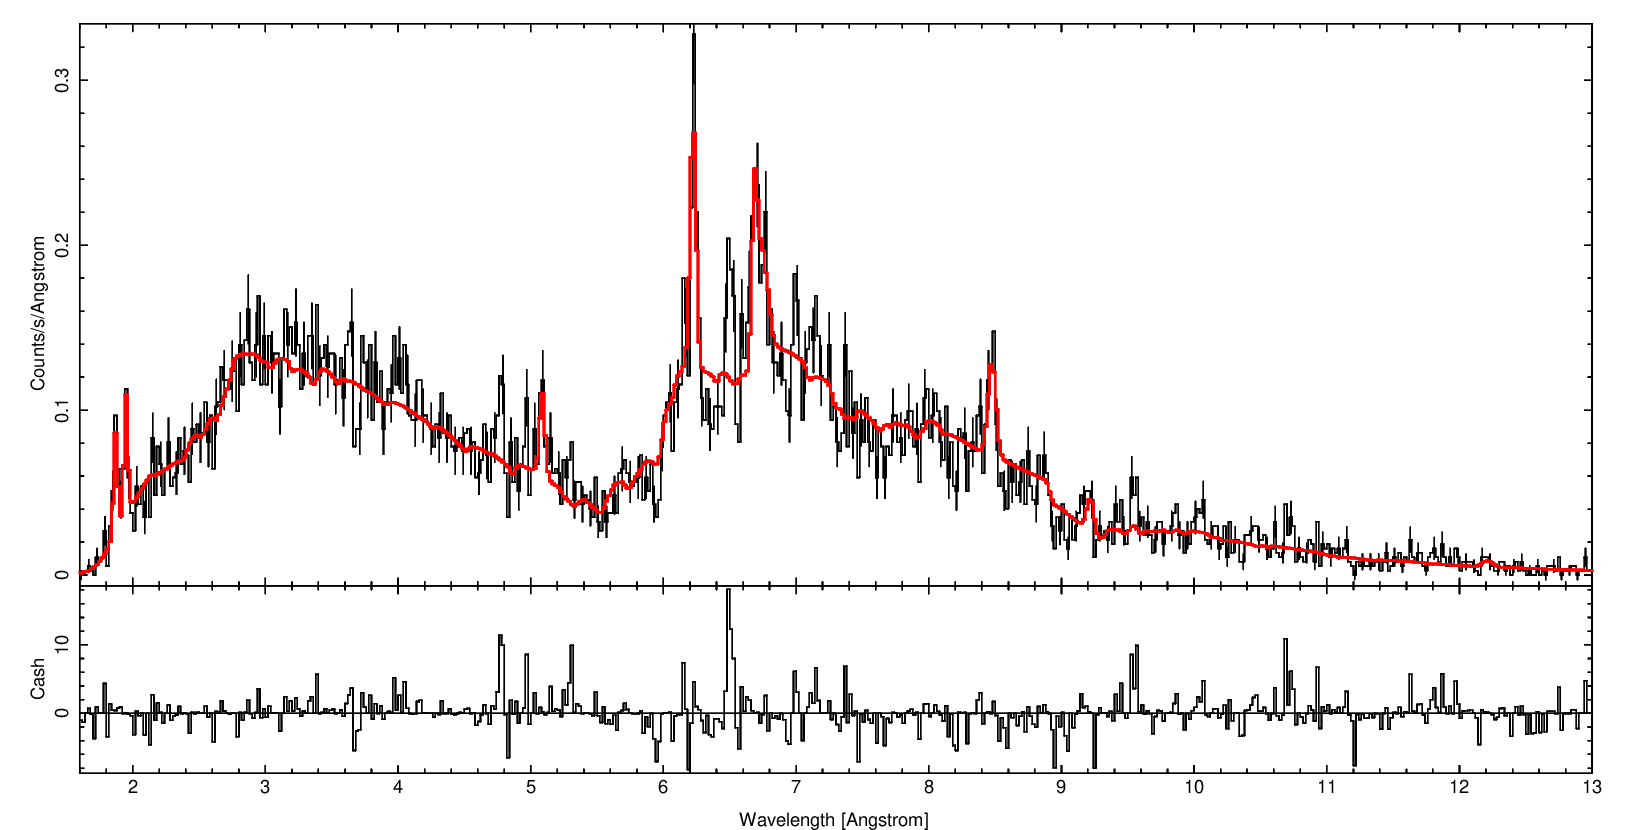
\includegraphics[width=1\linewidth]{Chapters/Figures/all_lines_fitted_meg.png}
    \caption{The fitted lines for the most prominent emissions in the MEG range}
    \label{fig:all_lines_2}
\end{figure}

Here are some zoomed-in graphs. See Fig~\ref{fig:zoomin2}, Fig~\ref{fig:zoomin1} and Fig~\ref{fig:zoomin3}

\begin{figure}[h!]
    \centering
    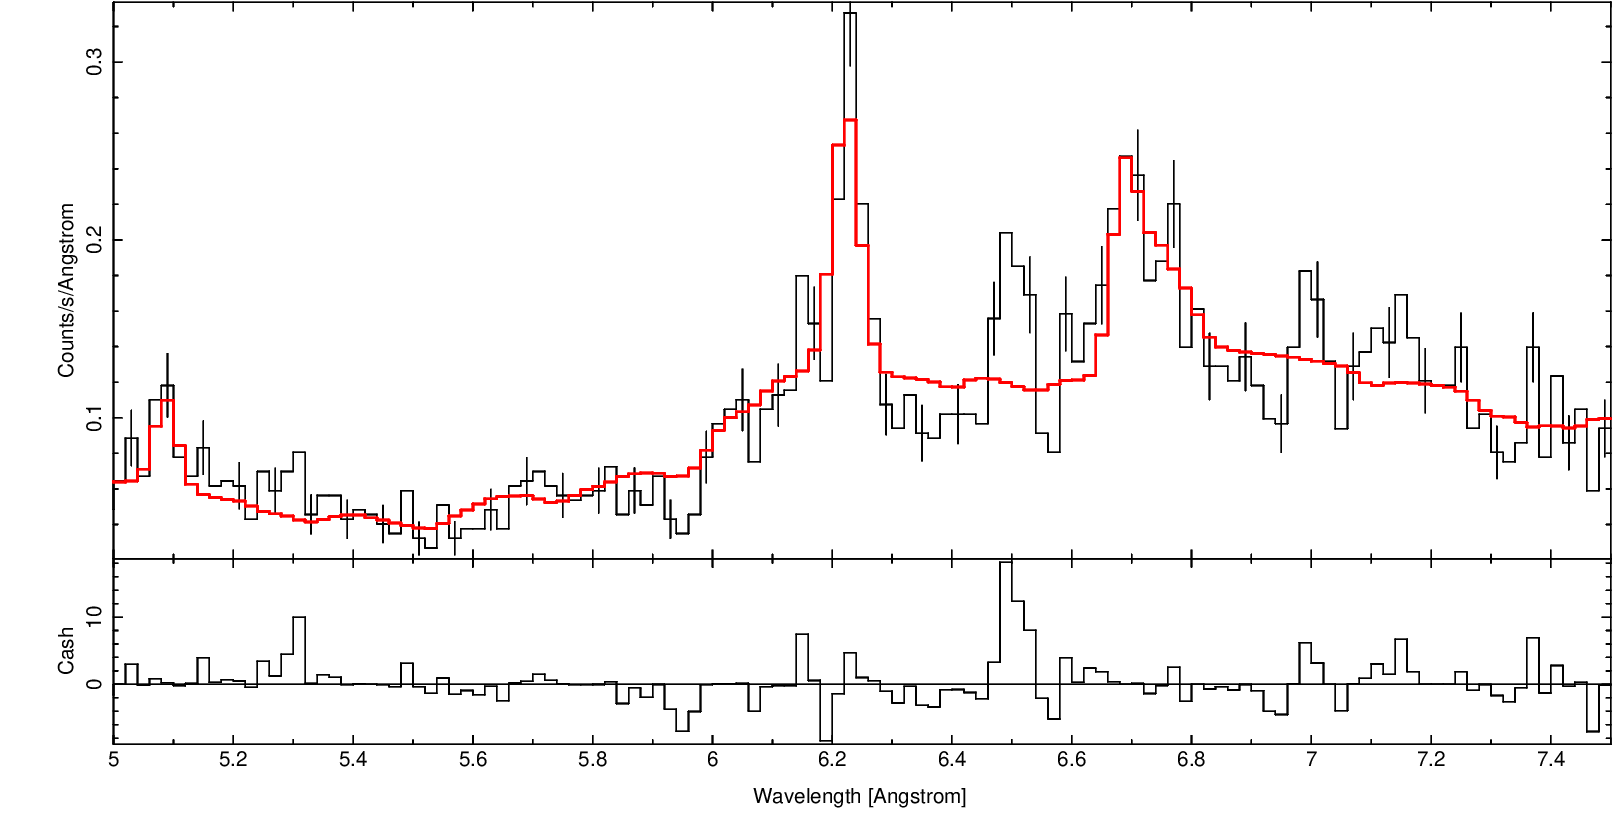
\includegraphics[width=1\linewidth]{Chapters/Figures/zoomin4.png}
    \caption{The zoom-in graph with perceived emission lines of S {\footnotesize\Romannum{15}}, Si {\footnotesize\Romannum{14}}, Si {\footnotesize\Romannum{13}r}, Si {\footnotesize\Romannum{13}i}, Si {\footnotesize\Romannum{13}f}}.
    \label{fig:zoomin2}
\end{figure}

\begin{figure}[h!]
    \centering
    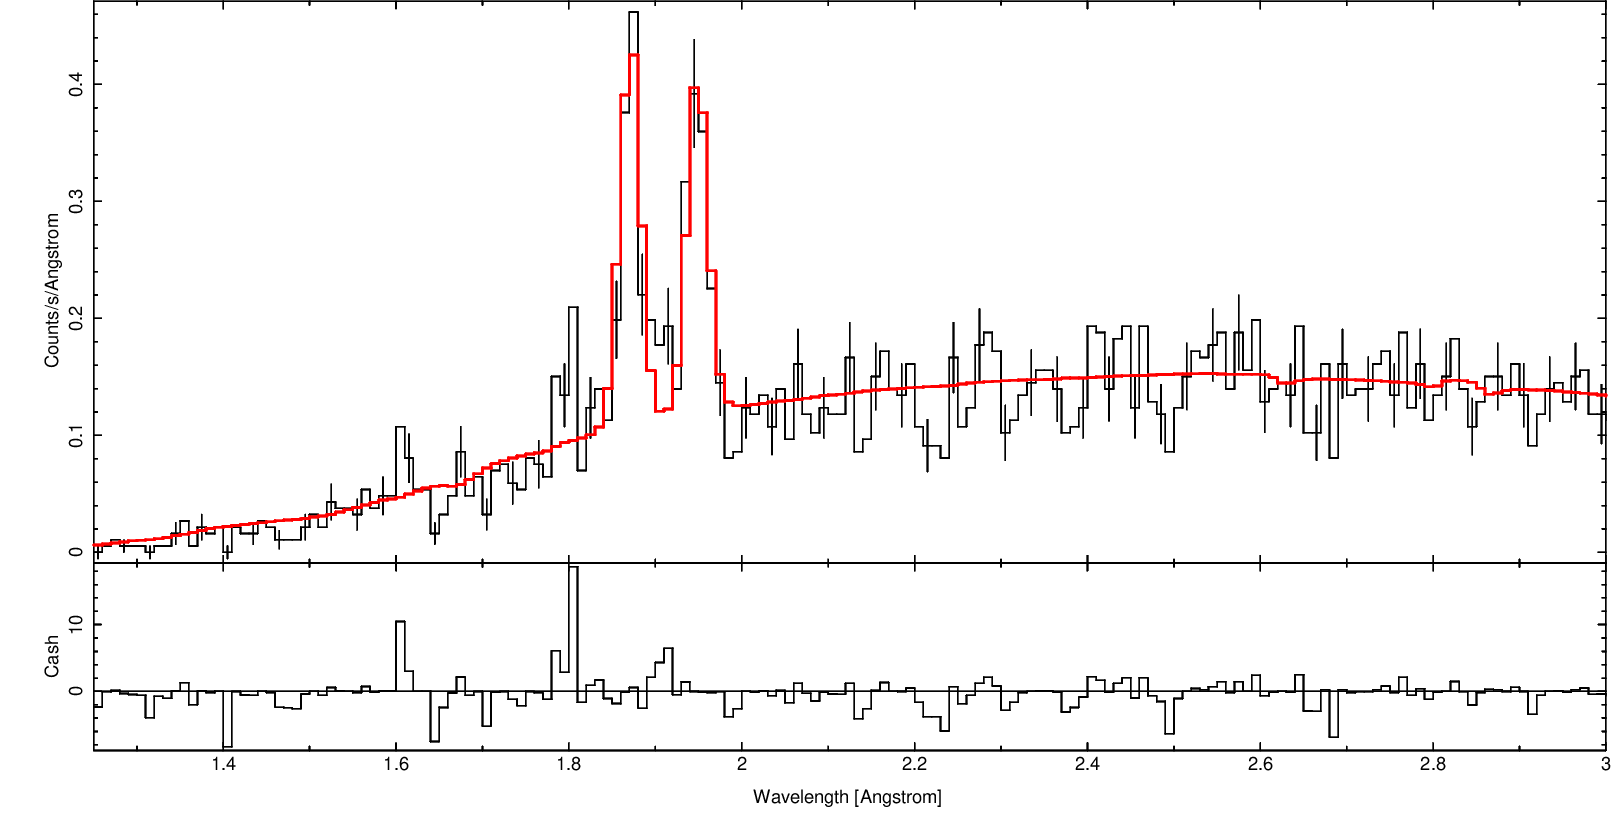
\includegraphics[width=1\linewidth]{Chapters/Figures/zoomin1.png}
    \caption{The zoom-in graph with perceived emission lines of Fe {\footnotesize\Romannum{26}}, Fe {\footnotesize\Romannum{25}}, and Fe {\footnotesize\Romannum{1}}}
    \label{fig:zoomin1}
\end{figure}


\begin{figure}[h!]
    \centering
    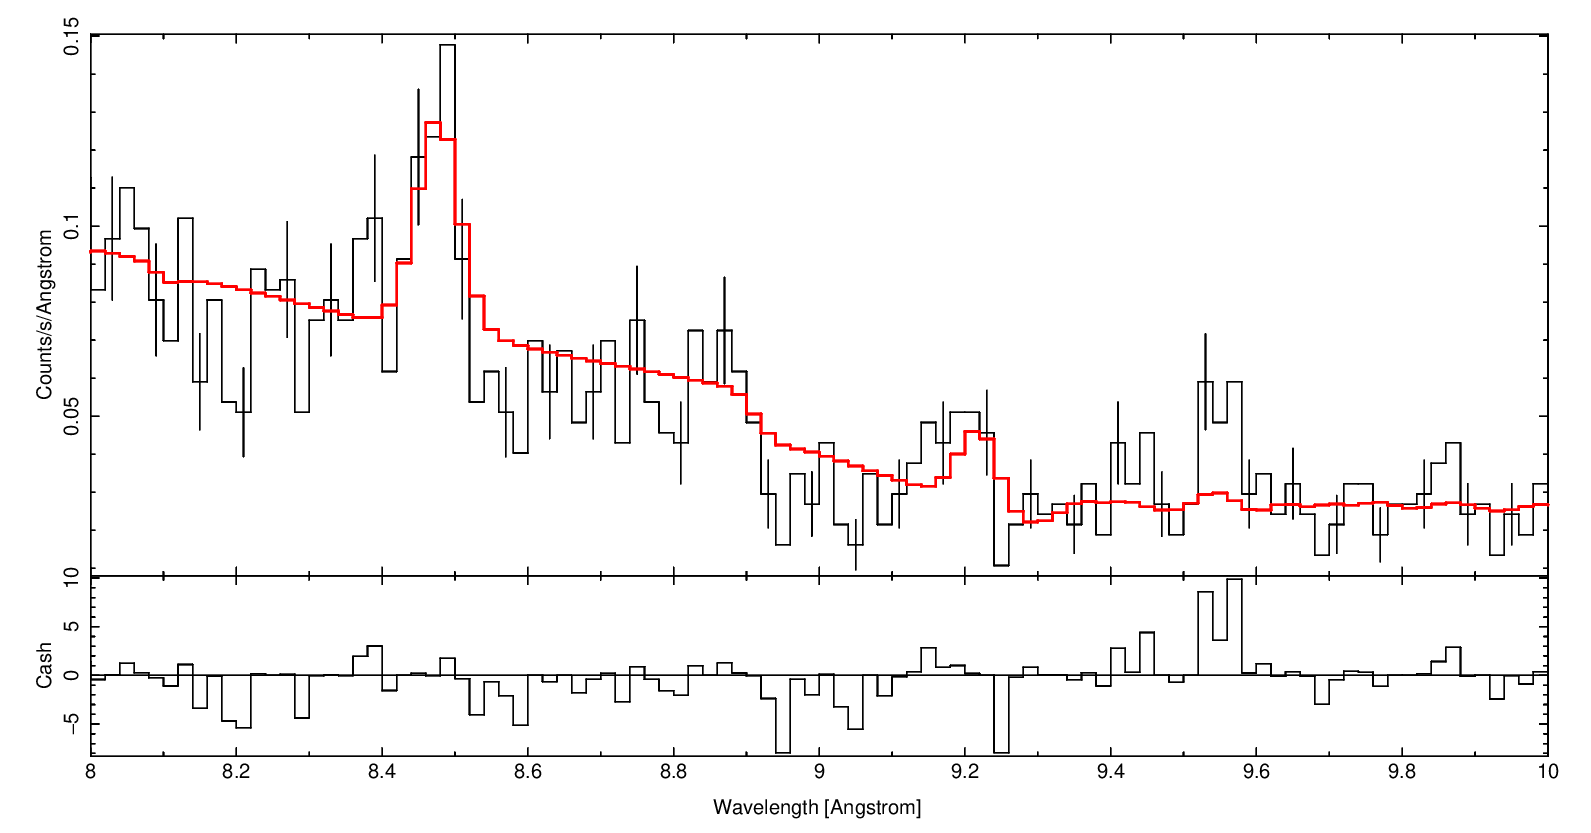
\includegraphics[width=1\linewidth]{Chapters/Figures/zoomin3.png}
    \caption{The zoom-in graph with perceived emission lines of Mg {\footnotesize\Romannum{12}}, and Mg {\footnotesize\Romannum{11}i}, Mg {\footnotesize\Romannum{11}r}, Mg {\footnotesize\Romannum{11}f}}.
    \label{fig:zoomin3}
\end{figure}

\clearpage

%\begin{verbatim}
    
\lstset{basicstyle=\footnotesize\ttfamily,breaklines=true}
\begin{lstlisting}[breaklines]
  idx  param     tie-to  freeze   value   min   max
  1  redshift(1).z    0   0  0.008250389   0.00825  0.009562  
  2  redshift(2).z    0   0   0.05083716  0.04  0.09  
  3  sigma(1).beta    0   0  0.003910095  0.0025  0.01  
  4  sigma(2).beta    0   0  0.006209743   0.005   0.015  
  5  wabs(1).nH     0   0  0.3721895     0  100000  10^22
  6  rest_wave(1).lambda  0   1     6.1823     0     0  
  7  rest_wave(2).lambda  0   1     8.4211     0     0  
  8  rest_wave(3).lambda  0   1    12.1351     0     0  
  9  rest_wave(4).lambda  0   1     5.0553     0     0  
 10  rest_wave(5).lambda  0   1    6.64795     0     0  
 11  rest_wave(6).lambda  0   1    6.68659     0     0  
 12  rest_wave(7).lambda  0   1    6.74029     0     0  
 13  rest_wave(8).lambda  0   1     1.8545     0     0  
 14  rest_wave(9).lambda  0   1     1.7799     0     0  
 15  rest_wave(10).lambda   0   1     9.1688     0     0  
 16  rest_wave(11).lambda   0   1     9.2297     0     0  
 17  rest_wave(12).lambda   0   1     9.3143     0     0  
 18  rest_wave(13).lambda   0   1     1.5883     0     0  
 19  rest_wave(14).lambda   0   1     1.8545     0     0  
 20  powerlaw(1).norm   0   0   0.01042019     0   1e+10  
 21  powerlaw(1).PhoIndex   0   0    0.93563    -2     9  
 22  gauss(1).area    0   0   0.0001349136     0     0  photons/s/cm^2
 23  gauss(1).center  0   1   6.233306     0    40  A
#=>  (1+redshift(1).z)*rest_wave(1).lambda
 24  gauss(1).sigma   0   1   0.02437282   1e-06     1  A
#=>  (1+redshift(1).z)*rest_wave(1).lambda*sigma(1).beta
 25  gauss(2).area    0   0   7.185216e-05     0     0  photons/s/cm^2
 26  gauss(2).center  0   1   8.490577     0    40  A
#=>  (1+redshift(1).z)*rest_wave(2).lambda
 27  gauss(2).sigma   0   1   0.03319897   1e-06     1  A
#=>  (1+redshift(1).z)*rest_wave(2).lambda*sigma(1).beta
 28  gauss(3).area    0   0   6.199978e-05     0     0  photons/s/cm^2
 29  gauss(3).center  0   1   12.23522     0    40  A
#=>  (1+redshift(1).z)*rest_wave(3).lambda
 30  gauss(3).sigma   0   1   0.04784087   1e-06     1  A
#=>  (1+redshift(1).z)*rest_wave(3).lambda*sigma(1).beta
 31  gauss(4).area    0   0   9.408116e-05     0     0  photons/s/cm^2
 32  gauss(4).center  0   1   5.097008     0    40  A
#=>  (1+redshift(1).z)*rest_wave(4).lambda
 33  gauss(4).sigma   0   1   0.01992979   1e-06     1  A
#=>  (1+redshift(1).z)*rest_wave(4).lambda*sigma(1).beta
 34  gauss(5).area    0   0   0.0001372658     0     0  photons/s/cm^2
 35  gauss(5).center  0   1   6.702798     0    40  A
#=>  (1+redshift(1).z)*rest_wave(5).lambda
 36  gauss(5).sigma   0   1   0.02620858   1e-06     1  A
#=>  (1+redshift(1).z)*rest_wave(5).lambda*sigma(1).beta
 37  gauss(6).area    0   0   2.145622e-05     0     0  photons/s/cm^2
 38  gauss(6).center  0   1   6.741757     0    40  A
#=>  (1+redshift(1).z)*rest_wave(6).lambda
 39  gauss(6).sigma   0   1   0.02636091   1e-06     1  A
#=>  (1+redshift(1).z)*rest_wave(6).lambda*sigma(1).beta
 40  gauss(7).area    0   0   1.301116e-05     0     0  photons/s/cm^2
 41  gauss(7).center  0   1     6.7959     0    40  A
#=>  (1+redshift(1).z)*rest_wave(7).lambda
 42  gauss(7).sigma   0   1   0.02657262   1e-06     1  A
#=>  (1+redshift(1).z)*rest_wave(7).lambda*sigma(1).beta
 43  gauss(8).area    0   0   0.0004757573     0     0  photons/s/cm^2
 44  gauss(8).center  0   1   1.948778     0    40  A
#=>  (1+redshift(2).z)*rest_wave(8).lambda
 45  gauss(8).sigma   0   1   0.01210141   1e-06     1  A
#=>  (1+redshift(2).z)*rest_wave(8).lambda*sigma(2).beta
 46  gauss(9).area    0   0   0.0004765693     0     0  photons/s/cm^2
 47  gauss(9).center  0   1   1.870385     0    40  A
#=>  (1+redshift(2).z)*rest_wave(9).lambda
 48  gauss(9).sigma   0   1   0.01161461   1e-06     1  A
#=>  (1+redshift(2).z)*rest_wave(9).lambda*sigma(2).beta
 49  gauss(10).area   0   0   6.577367e-05     0     0  photons/s/cm^2
 50  gauss(10).center   0   1   9.244446     0    40  A
#=>  (1+redshift(1).z)*rest_wave(10).lambda
 51  gauss(10).sigma  0   1   0.03614667   1e-06     1  A
#=>  (1+redshift(1).z)*rest_wave(10).lambda*sigma(1).beta
 52  gauss(11).area   0   0  -2.833654e-05     0     0  photons/s/cm^2
 53  gauss(11).center   0   1   9.305849     0    40  A
#=>  (1+redshift(1).z)*rest_wave(11).lambda
 54  gauss(11).sigma  0   1   0.03638675   1e-06     1  A
#=>  (1+redshift(1).z)*rest_wave(11).lambda*sigma(1).beta
 55  gauss(12).area   0   0   2.449444e-05     0     0  photons/s/cm^2
 56  gauss(12).center   0   1   9.391147     0    40  A
#=>  (1+redshift(1).z)*rest_wave(12).lambda
 57  gauss(12).sigma  0   1   0.03672028   1e-06     1  A
#=>  (1+redshift(1).z)*rest_wave(12).lambda*sigma(1).beta
 58  gauss(13).area   0   0   -1.86183e-05     0     0  photons/s/cm^2
 59  gauss(13).center   0   1   1.669045     0    40  A
#=>  (1+redshift(2).z)*rest_wave(13).lambda
 60  gauss(13).sigma  0   1   0.01036434   1e-06     1  A
#=>  (1+redshift(2).z)*rest_wave(13).lambda*sigma(2).beta
 61  gauss(14).area   0   0   0.0001318383     0     0  photons/s/cm^2
 62  gauss(14).center   0   1     1.8698     0    40  A
#=>  (1+redshift(1).z)*rest_wave(14).lambda
 63  gauss(14).sigma  0   1  0.007311097   1e-06     1  A
#=>  (1+redshift(1).z)*rest_wave(14).lambda*sigma(1).beta
\end{lstlisting}
%\end{verbatim}


% \begin{table}[t]
% \begin{tabular}{|p{1cm}||p{4cm}|p{2cm}|p{2cm}|p{2.5cm}|p{2cm}|p{2cm}| }
%   \hline
%   \multicolumn{7}{|c|}{Parameter Table} \\
%   \hline
%     idx & Parameter & tie-to & freeze & value & min & max\\
%     \hline
%     1 & redshift(1).z  &        0  &   0     &   0.0065721 &  -0.001094  &  0.018906  \\
%     2 & redshift(2).z    &      0   &  0    &   0.05084416  &      0.04   &     0.09\\  
%     3 & sigma(1).beta    &      0   &  0   &   0.003289482  &    0.0025    &    0.01  \\
%     4 & sigma(2).beta     &     0  &   0  &    0.005581536  &     0.005   &    0.015  \\
%     5 & wabs(1).nH     &        0  &   0   &     0.3711946  &     0     & 100000 $10^{22}$  \\
%     6 & rest\_wave(1).lambda  &  0  &   1   &     6.1823  &     0     &      0  \\
%     7 & rest\_wave(2).lambda  &  0  &   1    &    8.4211  &     0     &      0  \\
%     8 & rest\_wave(3).lambda  &  0    & 1   &     12.1351 &     0      &     0  \\
%     9 & rest\_wave(4).lambda  &  0   &  1     &   5.0553  &       0     &      0  \\
%     10 & rest\_wave(5).lambda &   0  &   1    &  6.64795  &       0     &      0  \\
%     11 & rest\_wave(6).lambda  &  0  &   1    & 6.68659  &  0    &       0  \\
%     12 &  rest\_wave(7).lambda &   0  &   1  &  6.74029  &    0      &     0  \\
%     13 &  rest\_wave(8).lambda  &  0  &   1  & 1.8545   &    0      &     0  \\
%     14 & rest\_wave(9).lambda  &  0  &   1   & 1.7799    & 0   &    0  \\
%     15 & rest\_wave(10).lambda &  0  &   1   &   9.1688    &  0  &    0  \\
%     16 & rest\_wave(11).lambda &  0  &   1   &  9.2297   &    0  &   0\\  
%     17 & rest\_wave(12).lambda &  0  &   1   &  
%     9.3143   &    0  &   0  \\
%     18 & rest\_wave(13).lambda &  0  &   1  & 1.5883   &    0  &   0  \\
%     19 & rest\_wave(14).lambda &  0  &   1  &     1.8545   &    0  &   0  \\

%   \end{tabular}
% \end{table}
\newpage
11/15
After we fit the lines, we found that there are some lines that are missed fitting. I added Fe26 with redshift 1 and S16 with redshift 1 and the fitted lines show up well. I added some labels on the line fitting graph. We found that Fe26 from the "red"/western jet is overlapping with Fe25 from the "blue"/eastern jet. Look at Fig~\ref{fig:labeled1} and Fig~\ref{fig:labeled2}
\begin{figure}[h!]
    \centering
    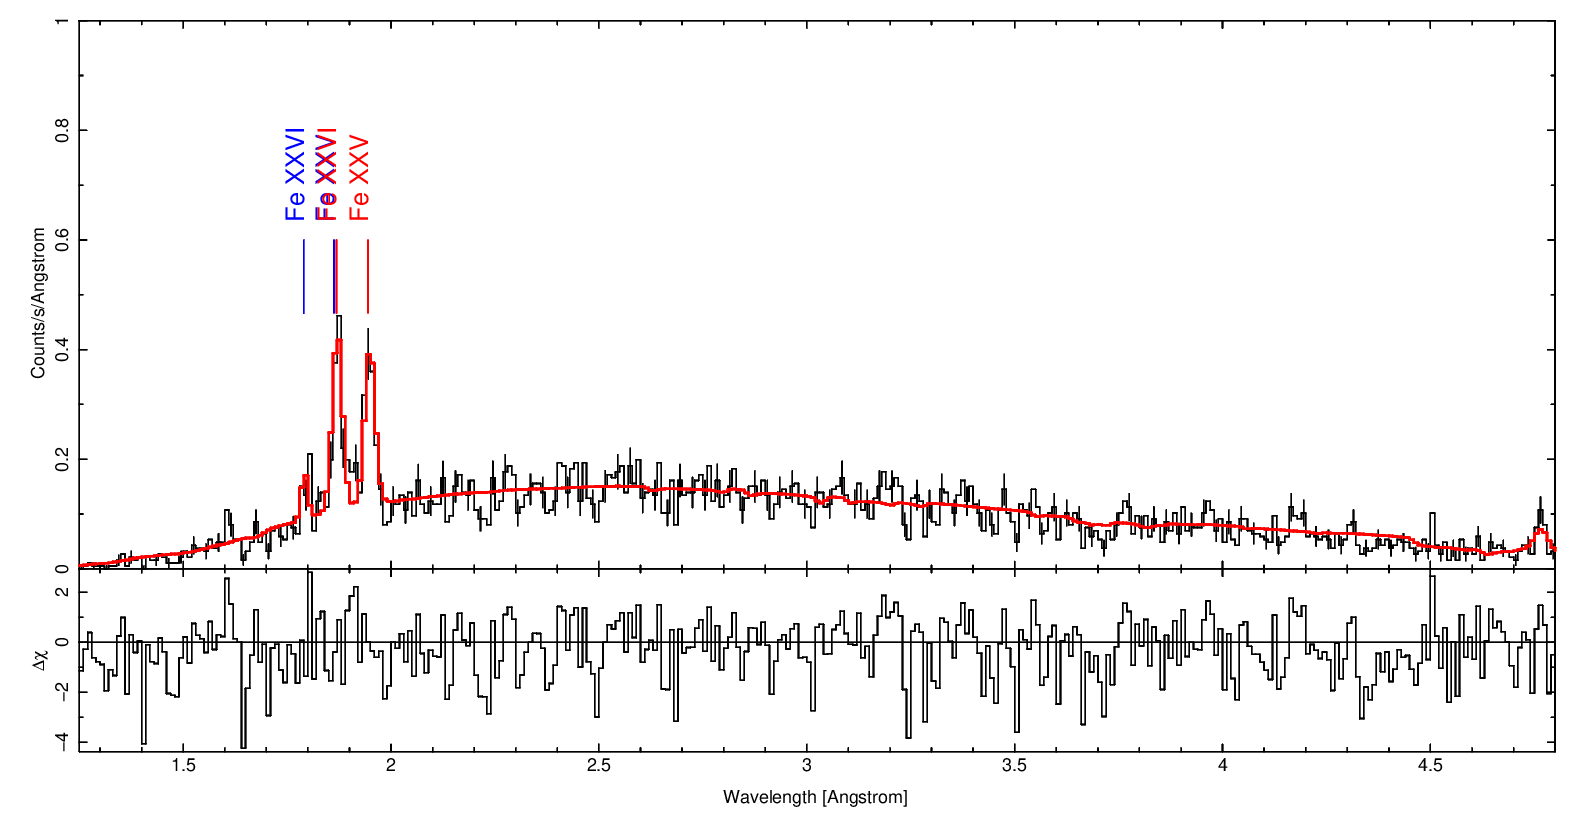
\includegraphics[width=0.9\linewidth]{Chapters/Figures/label1.png}
    \caption{The HEG spectrum of emission lines with labeled elements}.
    \label{fig:labeled1}
\end{figure}

\begin{figure}[h!]
    \centering
    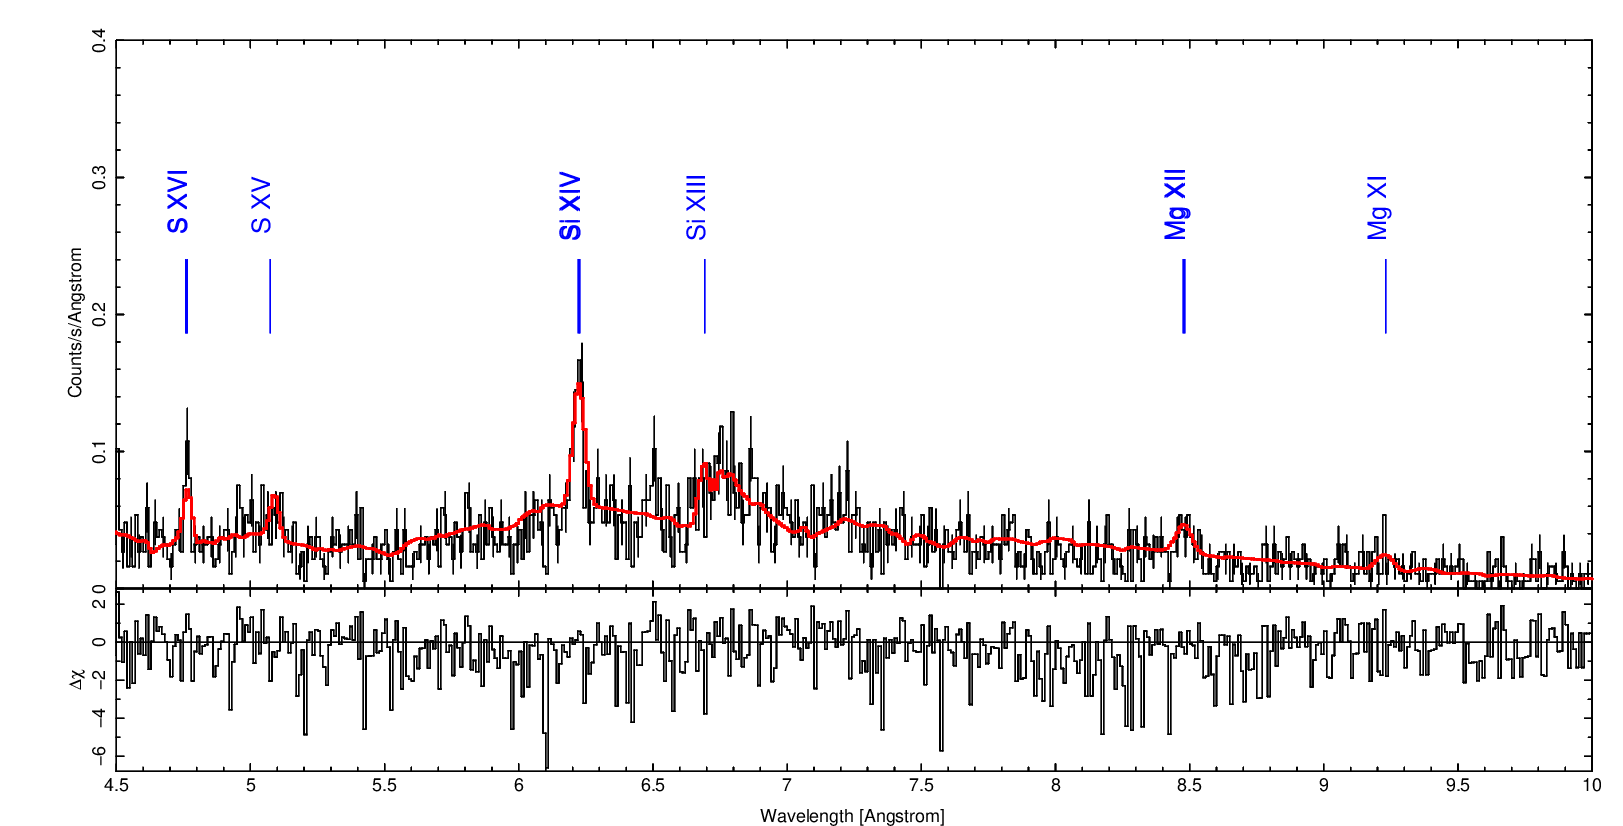
\includegraphics[width=0.9\linewidth]{Chapters/Figures/label2.png}
    \caption{The HEG spectrum of emission lines with labeled elements}.
    \label{fig:labeled2}
\end{figure}

\newpage
11/21\\
I ran the conf\_loop command for lines fit. The file that created by it is called pars\_allsave, which contains the confidence interval for all the parameters.\\
Questions to ask Herman:\\
In the code :
\begin{lstlisting}
load_par("par_9lines_g4.txt");
wline = [23,26,29,32,35,38,47,50,59,62];
nline = length(wline);
for(i=0;i<nline;i++) {
   idx = wline[i];
   gpi = get_par_info( idx );
   variable val=gpi.value;
   set_par(idx, val, 0, 0.3*val, 3.0*val);
}
\end{lstlisting}
Why we free those parameters that are for the Gaussian centers?

I loaded this save\_par file in the fit line script and look at the output plot and compare it with the previous one.\\
There is no big difference between two plots and I will check the plot with the parameter file and see where are those negative areas.\\

11/27
The three elements that have the negative area are restwave(11)[Mg11i], restwave(13)[Ni1], and restwave(14)[Fe25], which have line center at 9.292653 A, 1.669105 A, and 1.867149 A. By looking at the graph, I found the line center values in the parameter file does not exactly match the peak of the gaussian, which corresponds to a gap prior or after the peak.\\
I will free the line centers. Nothing changes.

Then I changed the values in the parameter file for the plasma model corresponding to the values that are found by the lines fit. And I start the cash fit and the conf loop.

11/28\\
The plasma fit finished. The fitting does not work well at the peak at about 1.95 and 1.5 - 1.8 range. 
Questions:\\
1. When the second jet is not tied to the first jet, how should we change the limit?\\
2. What parameters should we tie? 



11/29\\
Try to tweak the plasma model\\ 
How to set the range of the plasma model??\\

Jet with more emission lines (the jet with redshift ~ 0.0065 in our case) has smaller turbulence because the lines are narrower.\\

When I make the range of norms large, the width of the gaussian becomes large. 
When I manually increase the turbulence of jets the height of the peaks decrease. 
For the first jet, norm4 largely decides the height of the peak while norm1, 2, and 3 need to be increased a lot to see the change. 

 Look at Fig~\ref{fig:labeled1} and Fig~\ref{fig:labeled2}
 
 \newpage
\begin{figure}[h!]
    \centering
    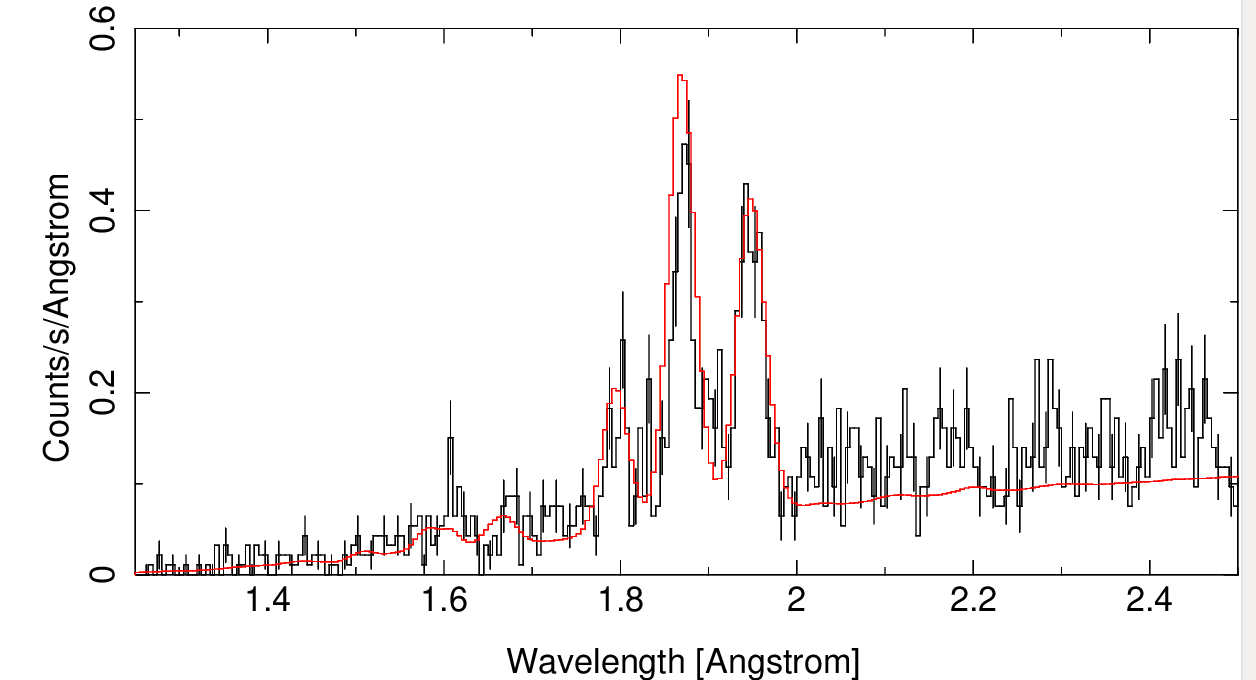
\includegraphics[width=0.9\linewidth]{Chapters/Figures/short_wavelength.png}
    \caption{The plasma fitting model for the longer wavelength range with manually twisted parameters}.
    \label{fig:manual_long}
\end{figure}

\begin{figure}[h!]
    \centering
    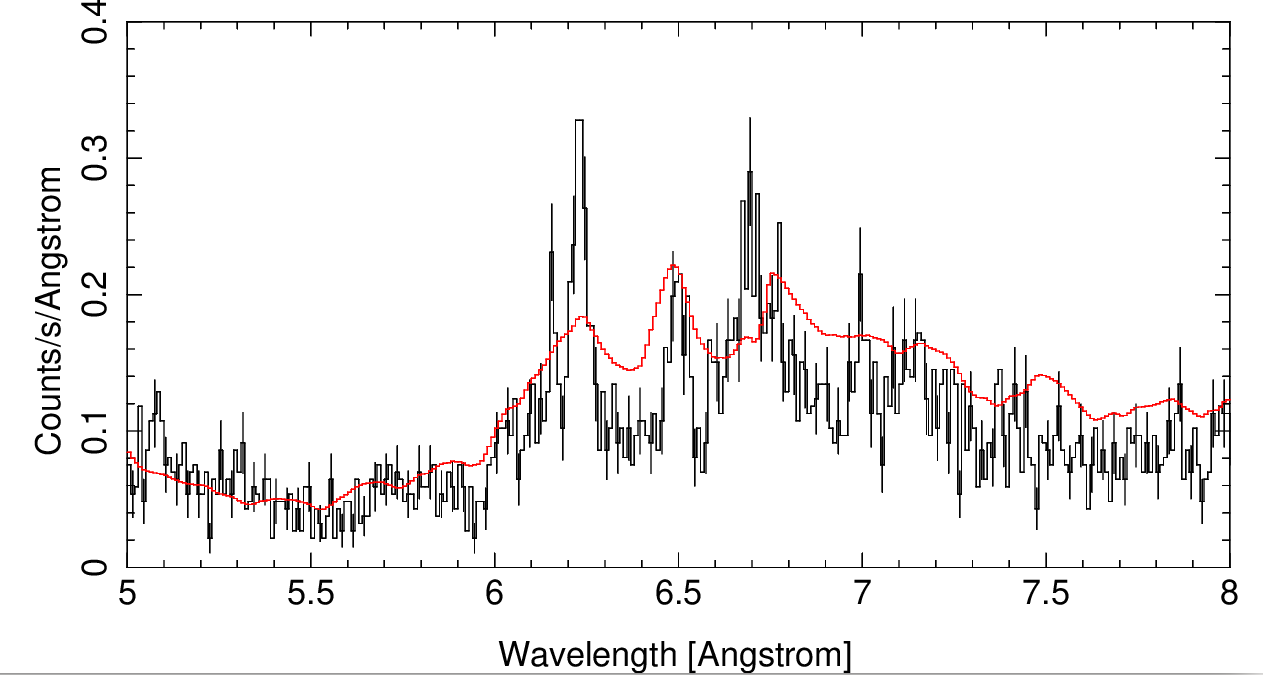
\includegraphics[width=0.9\linewidth]{Chapters/Figures/long_wavelength.png}
    \caption{The plasma fitting model for the shorter wavelength range with manually twisted parameters}.
    \label{fig:manual_short}
\end{figure}


12/3\\
Adding more lines in the line fit graph as Herman suggested in the latest email.\\
How to solve the problem of "continuum is too high, due (probably) to unmodeled lines"?\\

I tuned the parameters for plasma model and got better graphs.\\
Some notes:\\
1. norm1 for jet1 controls peak at 6.5-7 A.\\

12/11\\
I downloaded the longer observation 20131 from \url{https://cda.harvard.edu/chaser/mainEntry.do}

1/5\\
To create pha and mfa files, setup\_obsdir is needed to run. However, I cannot run setup\_obsdir {dir of observation} directly. Instead, I need to find where it is and run bash {dir of setup\_obsdir} observation. Might need to define sth. in .bashrc. \\
All files are created.\\



2/3\\
Use the head command to look at the event file in different parts of the long observation.\par

Mission Elapsed Time (MET) is used by NASA during their space missions, most notably during their Space Shuttle missions. Because so much of the mission depends on the time of launch, all events after launch are scheduled on the Mission Elapsed Time. This avoids constant rescheduling of events in case the launchtime slips. The MET-clock is set to zero at the moment of liftoff and counts forward in normal days, hours, minutes, and seconds.\\
MJD\_OBS =  5.8343629734065E+04 / Modified Julian date of observation \par
Found the Tstart and Tend in the evt0 file and calculated the time intervals of the four parts. Entered the time in XMM\/Chandra seconds since 1998.0 TT (decimal) on website \url{https://go.nasa.gov/2UIGMjk} to find the MJD.

\begin{table}[t]
\caption{The observation information for different parts of the long observation and expected red shifts}
\centering 
% used for centering table
\begin{tabular}{c c c c c}
\hline
\hline                       
Part & Starting Time & Ending Time & zred & zblue\\ [0.5ex]
\hline
0 & 58343.62893332 & 58343.85713227 & -0.009697 & 0.086842\\
1 & 58343.85713227 & 58344.08533122& -0.010609 & 0.087753\\
2 & 58344.08533122 & 58344.31353015 & -0.011065 & 0.0881213 \\
3 & 58344.31353015 & 58344.54172910 & -0.01105 & 0.088195\\
4 &  &  & -0.010572 & 0.087716\\
[1ex]
\hline
\end{tabular}
\label{table:nonlin}
\end{table}\par


2/5\\
Then I used the similar method that I did in the short observation to find the theoretical red-shifted and blue-shift wavelengths for 5 parts. Need to make a table for the rest wavelengths, observed wavelengths, and line flux.
2/9\\
I fit the lines for 5 parts and found that the red shift for the red jet is much larger than the theoretical one.\\

\begin{table}[t]
\caption{SS 433 Western Jet (smaller red shift) Lines}
\centering 
% used for centering table
\begin{tabular}{c c c  }
\hline
\hline                       
$\lambda_{rest}$ (\AA)& $\lambda_{obs}$ (\AA) & Flux ($10^{-6}$ photons cm$^{-2}$s$^{-1}$)\\ [0.5ex]
\hline
\multirow{7}{4em}{6.1823} & 6.406382 & 0.0001953477\\
 & 8.726329 & 8.070485e-05\\
\multirow{7}{4em}{6.64795} & 6.88891 & 0.0001081967\\
\multirow{7}{4em}{6.68659} & 6.928951 & 1.038041e-05\\
\multirow{7}{4em}{6.74029} & 6.984597 & 1.630129e-05\\
\multirow{7}{4em}{5.0553} & 5.238533 & 9.152973e-05\\
\multirow{7}{4em}{1.592} & 1.649703 & 0.0002589697\\
\multirow{7}{4em}{1.8545} & 1.921718 & 0.001026132\\
\multirow{7}{4em}{1.7799} & 1.844414 & 0.0002451663\\
\multirow{7}{4em}{9.1688} & 9.50113 & 3.047942e-05\\
\multirow{7}{4em}{9.2297} & 9.564238 & 1.607879e-06\\
\multirow{7}{4em}{9.3143} & 9.651904 & 4.382468e-05\\
\multirow{7}{4em}{4.73} & 4.901442 & 0.0001567437\\
\multirow{7}{4em}{6.64795} & 7.185847 & 3.4199e-05\\
\multirow{7}{4em}{6.68659} & 7.227614 & -6.881935e-05\\
\multirow{7}{4em}{6.74029} & 7.285659 & 5.898873e-05\\
\multirow{7}{4em}{6.1823} & 6.682521 & 7.490763e-05\\
 & 6.400339 & 0.0002093213\\
 & 8.718098 & 9.722996e-05\\
 & 6.882412 & 9.122088e-05\\
 & 6.922415 & 1.795798e-05\\
 & 6.978009 & 4.944435e-05\\
\multirow{7}{4em}{8.4211}& 5.233592 & 9.761647e-05\\
 & 1.648147 & 0.0002369767\\
 & 1.919905 & 0.0008224793\\
 & 1.842674 & 0.0002559987\\
 & 9.492168 & 3.505377e-05\\
 & 9.555216 & -2.071569e-05\\
 & 9.642799 & 2.584576e-05\\
 & 4.896819 & 0.0001333559\\
 & 7.189345 & -6.182377e-07\\
 & 7.231132 & -4.983215e-05\\
 & 7.289205 & 4.465996e-05\\
 & 6.685774 & 7.39148e-05\\
 & 6.400427 & 0.0001816885\\
 & 8.718218 & 7.379159e-05\\
 & 6.882506 & 8.407732e-05\\
 & 6.92251 & 1.787087e-05\\
 & 6.978104 & 4.133396e-05\\
 & 5.233664 & 9.000698e-05\\
 & 1.64817 & 0.0002635255\\
 & 1.919931 & 0.0007689837\\
 & 1.842699 & 0.0002975289\\
 & 9.492298 & 6.446505e-06\\
 & 9.555347 & 1.417067e-05\\
 & 9.642932 & -3.449051e-06\\
 & 4.896886 & 0.0001191925\\
 & 7.189102 & -3.62957e-05\\
 & 7.230887 & 1.030425e-05\\
 & 7.288959 & 2.429657e-05\\
 & 6.685547 & 4.134544e-05\\
 & 6.400808 & 0.0002132997\\
 & 8.718736 & 5.533479e-05\\
 & 6.882916 & 7.374446e-05\\
 & 6.922921 & 2.188877e-05\\
 & 6.978519 & 5.132219e-05\\
 & 5.233975 & 6.269798e-05\\
 & 1.648268 & 0.0002554855\\
 & 1.920046 & 0.0008173814\\
 & 1.842809 & 0.0002206411\\
 & 9.492863 & 5.745678e-05\\
 & 9.555915 & -2.604159e-05\\
 & 9.643505 & 4.019557e-05\\
 & 4.897177 & 0.0001415489\\
 & 7.202428 & 4.392368e-05\\
 & 7.244291 & -0.0001021545\\
 & 7.30247 & 0.0001004292\\
 & 6.69794 & 7.134898e-05\\
 & 6.396571 & 0.0002129926\\
 & 8.712965 & 7.42718e-05\\
 & 6.87836 & 8.21608e-05\\
 & 6.918339 & 1.370373e-05\\
 & 6.9739 & 5.211237e-05\\
 & 5.230511 & 0.0001347571\\
 & 1.647177 & 0.0001451571\\
 & 1.918775 & 0.0008333993\\
 & 1.841589 & 0.0003086422\\
 & 9.48658 & 7.023839e-05\\
 & 9.54959 & -5.605822e-05\\
 & 9.637123 & 4.592911e-05\\
 & 4.893936 & 0.0001474191\\
 & 7.218701 & 4.583201e-07\\
 & 7.260659 & -8.00107e-05\\
 & 7.318969 & 9.137724e-05\\
 & 6.713073 & 5.978347e-05\\
[1ex]
\hline
\end{tabular}
\label{table:nonlin}
\end{table}\par



\begin{figure}[h!]
    \centering
    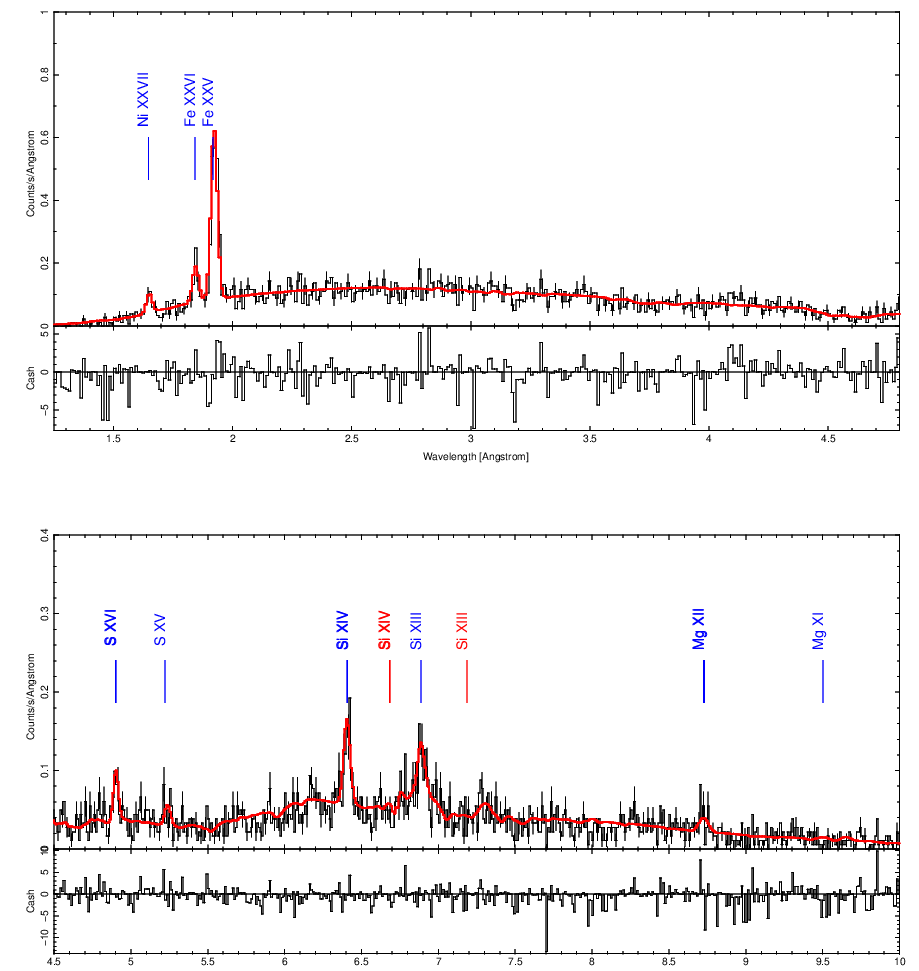
\includegraphics[width=\linewidth]{Chapters/Figures/part0_heg.png}
    \caption{The line fit graph for the HEG spectrum of part 0 of the long observation}
    \label{fig:part0}
\end{figure}

\begin{figure}[h!]
    \centering
    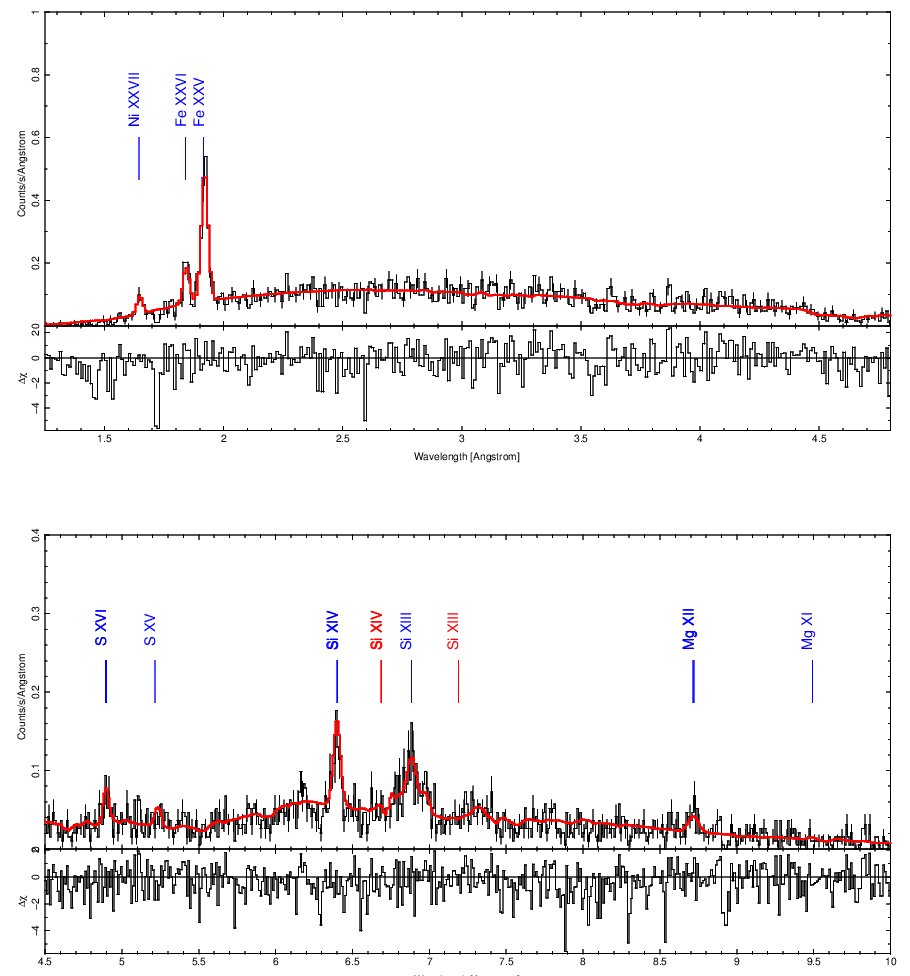
\includegraphics[width=\linewidth]{Chapters/Figures/part1_heg.png}
    \caption{The line fit graph for the HEG spectrum of part 1 of the long observation}
    \label{fig:part1}
\end{figure}

\begin{figure}[h!]
    \centering
    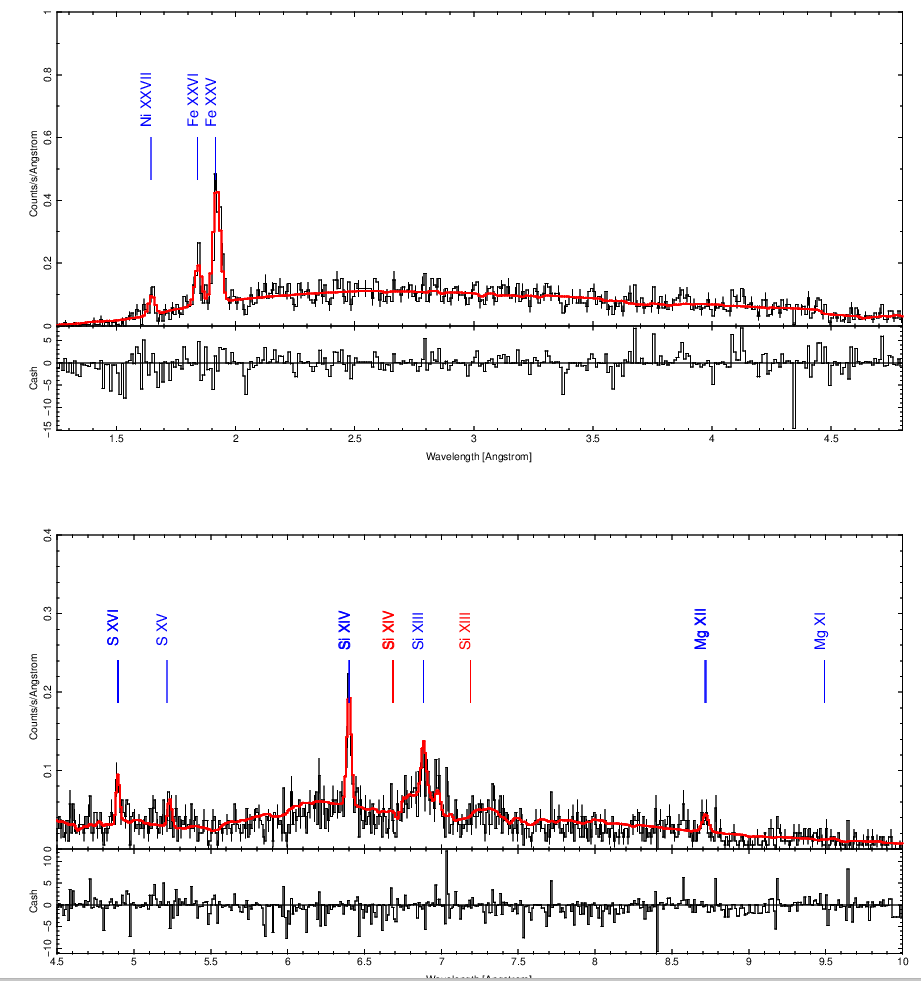
\includegraphics[width=\linewidth]{Chapters/Figures/part2_heg.png}
    \caption{The line fit graph for the HEG spectrum of part 2 of the long observation}
    \label{fig:part2}
\end{figure}

\begin{figure}[h!]
    \centering
    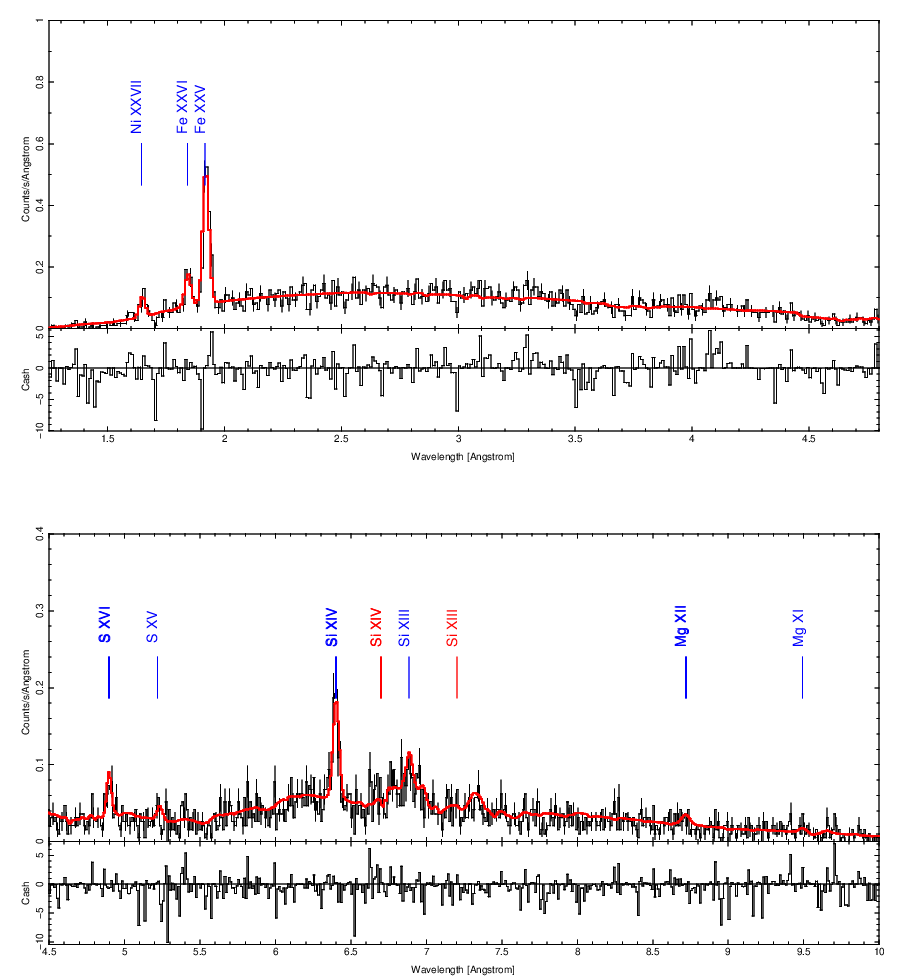
\includegraphics[width=\linewidth]{Chapters/Figures/part3_heg.png}
    \caption{The line fit graph for the HEG spectrum of part 3 of the long observation}
    \label{fig:part3}
\end{figure}

\begin{figure}[h!]
    \centering
    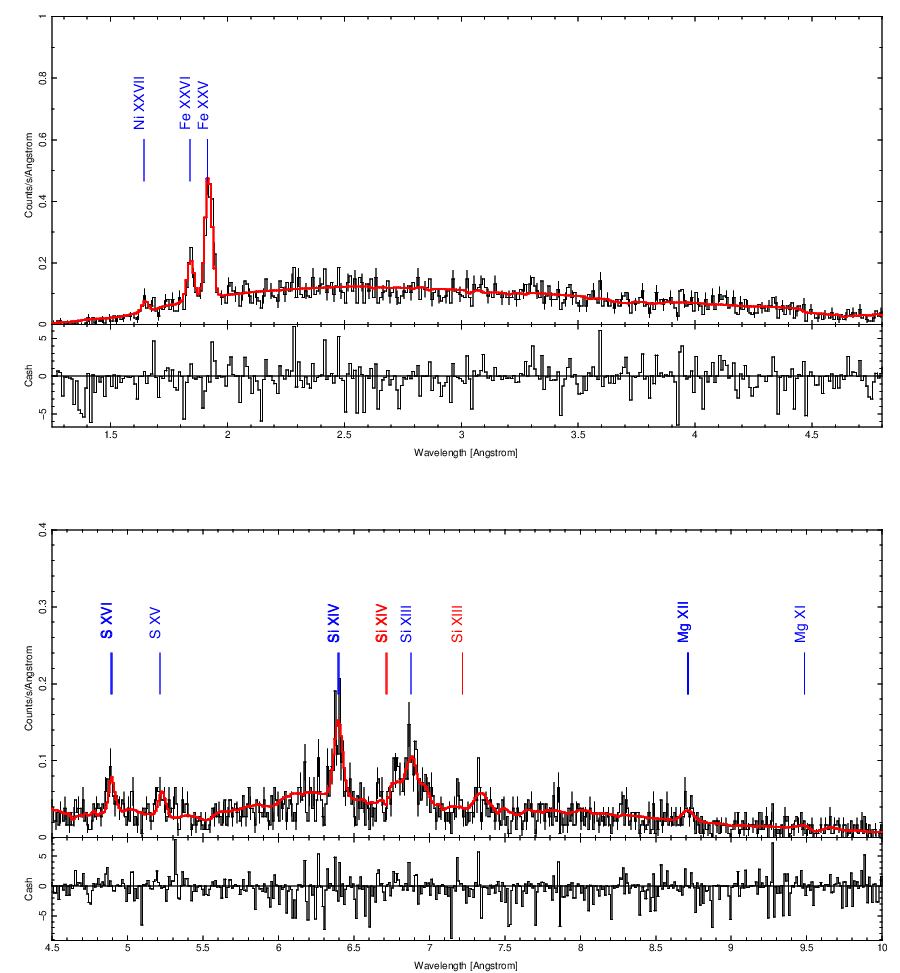
\includegraphics[width=\linewidth]{Chapters/Figures/part4_heg.png}
    \caption{The line fit graph for the HEG spectrum of part 4 of the long observation}
    \label{fig:part4}
\end{figure}



3/2\\
I am making the following graphs:\par
1. Observed redshift changes during 5 periods of the long observation comparing to the theoretical values; the redshifts from the short observation is also plotted.\par
2. Observed flux changes of emission lines from both jets (two plots) over time. Compare the flux change of these lines with the corresponding ones in the short observation.\par

One thing needs to be aware of is that Fe26 (from blue jet) and Fe25 (from red jet) overlap in the short observation. Since Fe25 (from the red jet) is fit first, the flux is significant. And thus the flux of Fe26 (from the blue jet) is small, even becomes negative. Therefore, I plot the flux as 0 for Fe26\par

For the long observation, there is only a few lines are from the blue jet. View Si13rif as a whole thing, is it ok?

3/3\\
For Fe 25 in the red jet, since its value is uncertain in the short observation, its fitted value is a negative number with large errors. I plotted it as 0 in the short observation.\par
Is it possible that we mix up the two jets?\par

3/24\\
I made the plot of the power-law spectra over the long observation. Instead of the fact that the normalization of the spectra increase due to accretor coming out of the eclipse, the normalization actually decreases over 5 parts. The spectra slope (photon index) first increases and then decreases. \par
Now I am going to use another method to test the redshift values. Put a gaussian at places where I think there should be a line and let ISIS to fit, then check what would be the wavelength.





\clearpage{}
\section{Some Linux command}
\# compile and run c files including math library\\
\textbf{gcc filename.c -lm}\\
\# extract .tar file\\
\textbf{tar -xvf}\\
\# extact tar.gz file\\
\textbf{tar -xzf *.tar.gz}\\
\# extract .gz file\\
\textbf{gunzip *.gz}\\
\# .bashrc is a shell script that Bash runs whenever it is started interactively. It initializes an interactive shell session. You can put any command in that file that you could type at the command prompt.\\
\textbf{gedit .bashrc}\\
\# Look at a pdf file\\
\textbf{xdg-open filename.xxx}
\# Transpose a file
\textbf{datamash --no-strict transpose < table.txt}\\



